\hypertarget{cv:gestionarAcciones}{\section{Gestionar Acciones}} \label{sec:GestionarAcciones}

	Esta funcionalidad le permitirá las acciones necesarias para controlar las acciones pertenecientes a una pantalla y visualizarlos en una tabla en el proyecto sobre el que se está operando y solicitar el registro de uno nuevo. Para entrar a esta gestión es necesario que al menos exista una pantalla dentro del proyecto.

		\subsection{Procedimiento}

			%Pasos de procedimiento
			\begin{enumerate}
				
			\item Ingrese a un proyecto existente desde la pantalla \ref{fig:GestionarProyectosColaborador}.
	
			\item Oprima el botón \IUPantallas{} de algún registro existente de la pantalla \ref{fig:GestionarModulos} ''Gestionar Módulos''.
			
			\item Oprima el botón \IUAcciones{} de algún registro existente de la pantalla \ref{fig:GestionarPantallas} ''Gestionar Pantallas''.
			
			\item \item Se mostrará la pantalla \ref{fig:GestionarAcciones} ''Gestionar Acciones''.

			%Pantalla
			\begin{figure}[h!]
				\begin{center}
					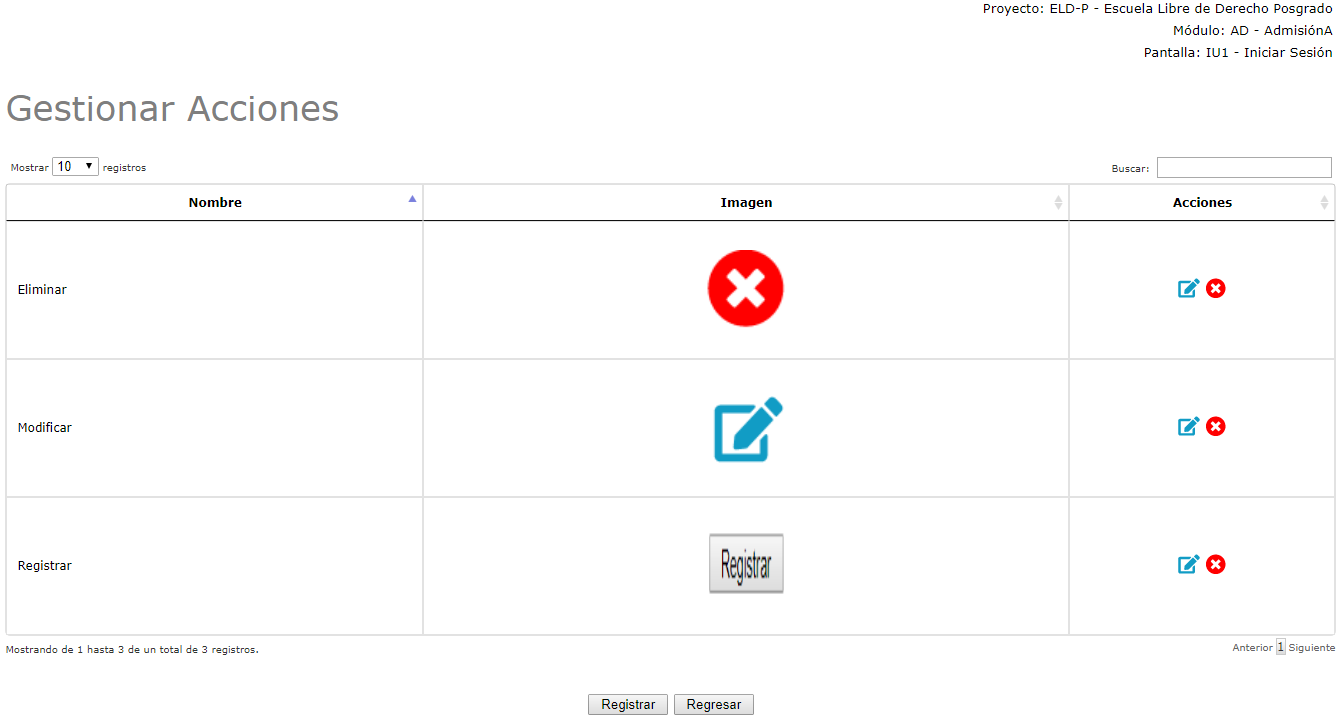
\includegraphics[scale=0.5]{roles/lider/pantallas/acciones/pantallas/IU11-1-1gestionarAcciones}
					\caption{Gestionar Acciones}
					\label{fig:GestionarAcciones}
				\end{center}
			\end{figure}
		
				\item Seleccione la operación que desea realizar:
			
			Para (\hyperlink{cv:registrarAccion}{Registrar}) dé clic en el botón \IURegistrar.
			
			Para (\hyperlink{cv:modificarAccion}{Modificar}) dé clic en el icono \IUEditar{} de alguna acción ya registrada.
			
			Para (\hyperlink{cv:eliminarAccion}{Eliminar}) dé clic en el icono \IUBotonEliminar{} de alguna acción ya registrada.
			
			\end{enumerate}